\begin{figure}[t]
    \centering
    \begin{subfigure}[t]{1\linewidth}
        \centering
        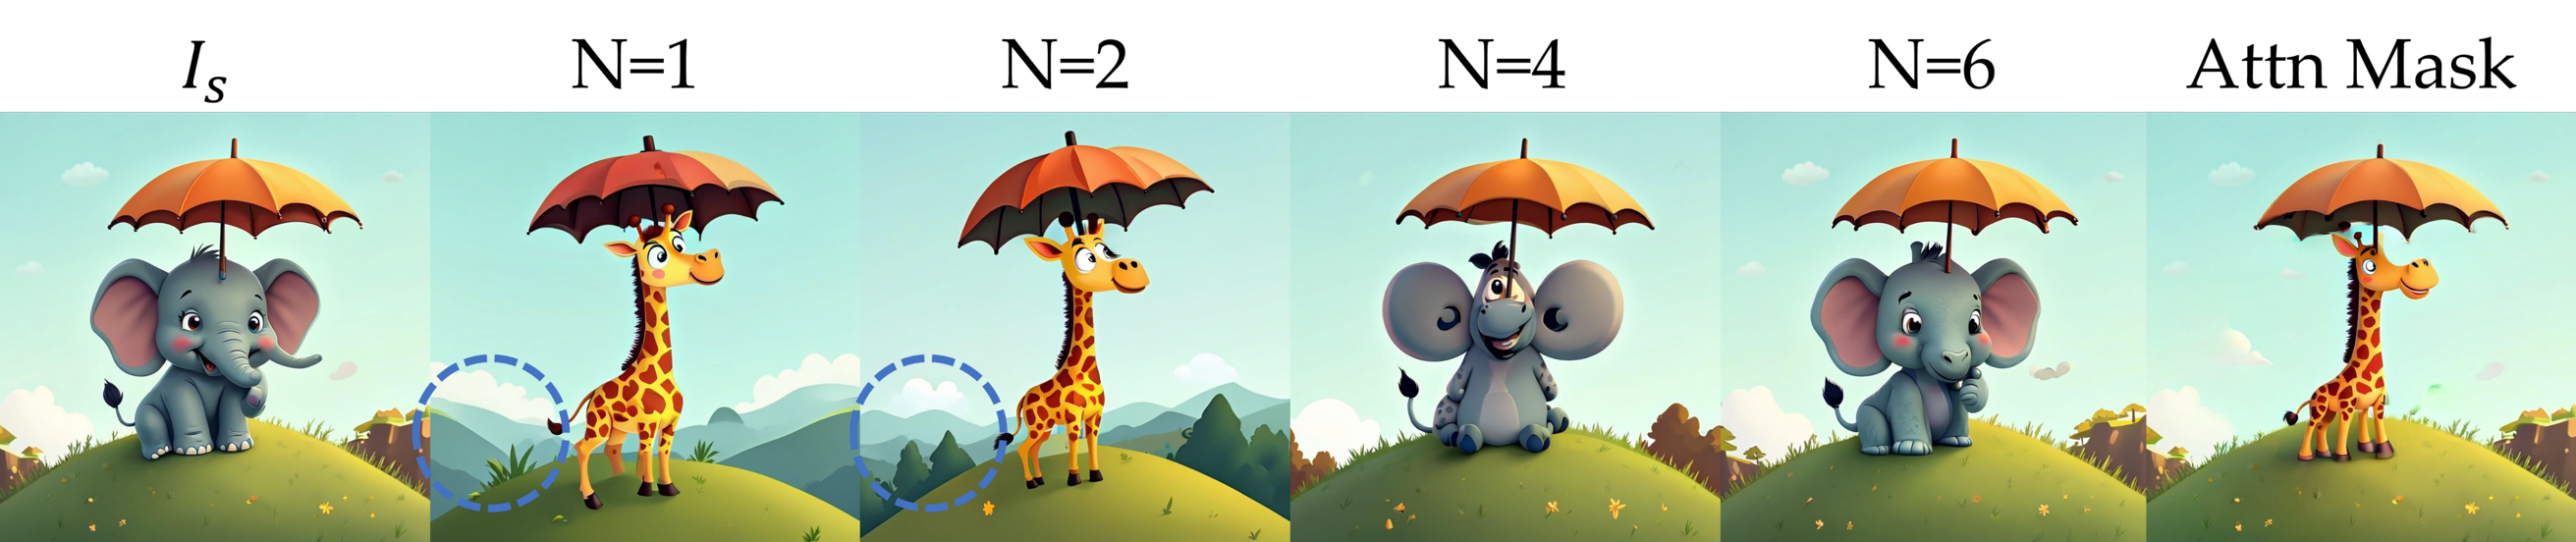
\includegraphics[width=\linewidth]{imgs/shape_diff.png}
        \caption{Scale-$N$ replacement: few shared scales allow editing but lose the background; many shared scales preserve the background but lock the subject. Our attention-mask approach achieves both precise editing and faithful preservation.}
        \label{fig:shape_diff_a}
    \end{subfigure}
    \hfill
    \begin{subfigure}[t]{1\linewidth}
        \centering
        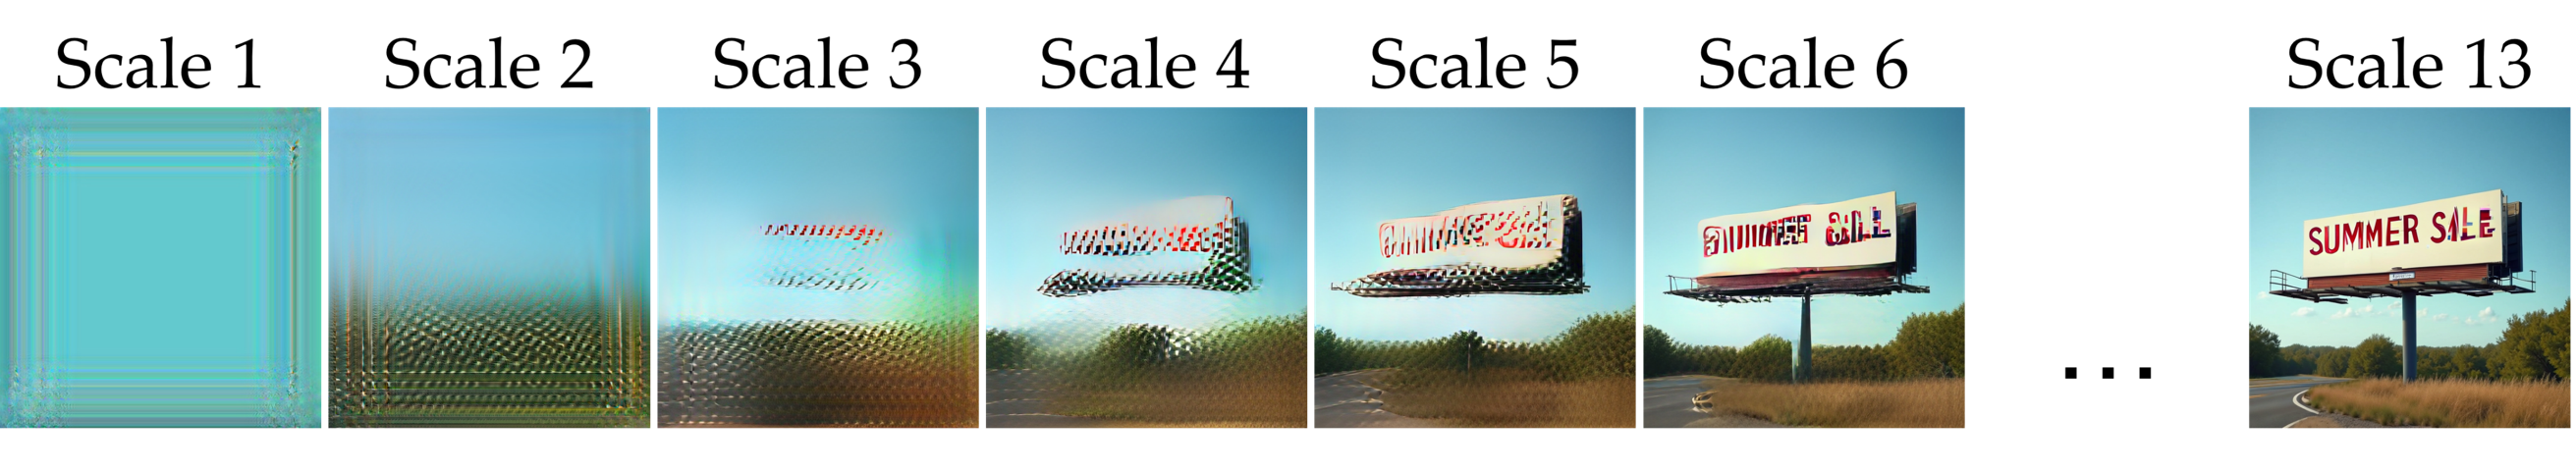
\includegraphics[width=\linewidth]{imgs/coarse2fine.png}
        \caption{VAR's coarse-to-fine generation: early scales ($k \leq 4$) determine global layout; later scales refine texture. Fixed-scale replacement thus cannot accommodate shape-changing edits.}
        \label{fig:shape_diff_b}
    \end{subfigure}
    \caption{Analysis of scale-level replacement vs.\ attention-based masking. (a) Comparison across configurations on an elephant $\to$ giraffe edit. (b) VAR's coarse-to-fine generation: early scales commit to global layout, limiting the effectiveness of fixed-scale replacement strategies.}
    \label{fig:shape_diff}
\end{figure}